\documentclass{beamer}

\usepackage[frenchb]{babel}
\usepackage[T1]{fontenc}
\usepackage[latin9]{inputenc}
\usepackage{graphicx}

\usetheme{CambridgeUS}




\AtBeginSection[]
{
  \begin{frame}
  \frametitle{Sommaire}
  \tableofcontents[currentsection]
  \end{frame} 
}


\title[1ere Soutenance Projet]{Soutenance mi-parcourt}
\author{Equipe CFR}
\institute{ESILV}
\date{16 janvier}



\begin{document}

%%%%%%%%%%%%%%
%%% diapo 1 %%
%%%%%%%%%%%%%%

\begin{frame}
\titlepage
\begin{center}

\includegraphics[width=3cm]{img/Logo_ESILV.png}
\end{center}
\end{frame}
	

\section{Qui nous sommes ?}
\subsection{Notre �quipe}


%%%%%%%%%%%%%%
%%% diapo 2 %%
%%%%%%%%%%%%%%


\begin{frame}
\frametitle{Une �quipe de folie !}
\begin{block}{}
\begin{itemize}
\item 12 �tudiants de l'�cole ESILV
\item Etudiants 2�me ann�e / 3�me ann�e 
\item Etudiants motiv�s 
\item Mentor en cours de th�se
\end{itemize}
\end{block}
\begin{center}
\end{center}
\end{frame}



\subsection{Notre association}


%%%%%%%%%%%%%%
%%% diapo 3 %%
%%%%%%%%%%%%%%


\begin{frame}
\frametitle{DaVinciBot, associtation de robotique}
\begin{center}

\includegraphics[height=3cm]{img/logo_assos.png}
\end{center}
\begin{block}{le but de l'association}
\begin{itemize}
\item G�rer les d�penses
\item Recevoir l'aide de sponsors
\end{itemize}
\end{block}
\end{frame}



\section{Coupe de France Robotique}
\subsection{Le d�roulement}


%%%%%%%%%%%%%%
%%% diapo 4 %%
%%%%%%%%%%%%%%

\begin{frame}
\begin{columns}
\begin{column}{0.3\textwidth}
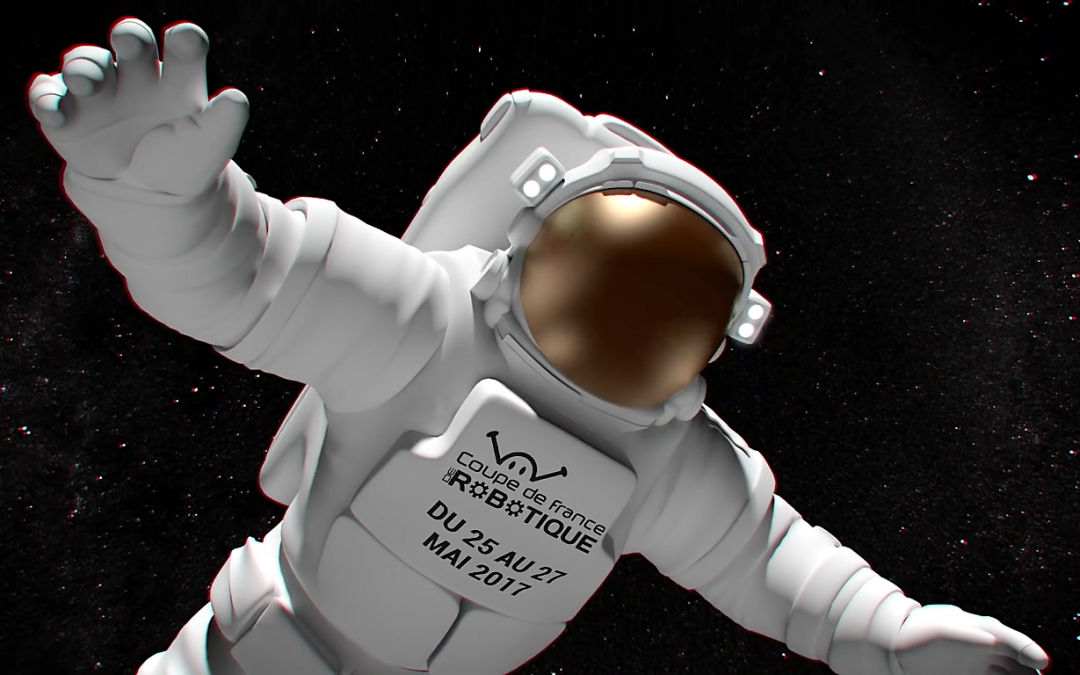
\includegraphics[width=3cm]{img/lune_pres.png}
\end{column}
\begin{column}{0.3\textwidth}

\includegraphics[width=3cm]{img/logo_coupe.jpg}
\end{column}
\begin{column}{0.3\textwidth}
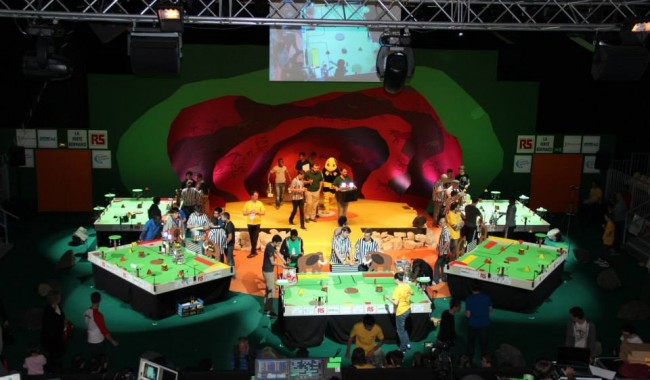
\includegraphics[width=3cm]{img/photo_coupe02.jpg}
\end{column}
\end{columns}
\begin{columns}
\begin{column}{0.4\textwidth}
\begin{block}{La coupe !}
\begin{itemize}
\item 200 �quipes
\item Syst�me de battle 
\item 90 secondes 
\item th�me : la lune 
\item 25 au 27 mai 20167
\item Roche-sur-Yon 
\end{itemize}
\end{block}
\end{column}
\begin{column}{0.4\textwidth}
\vspace{0.5cm}
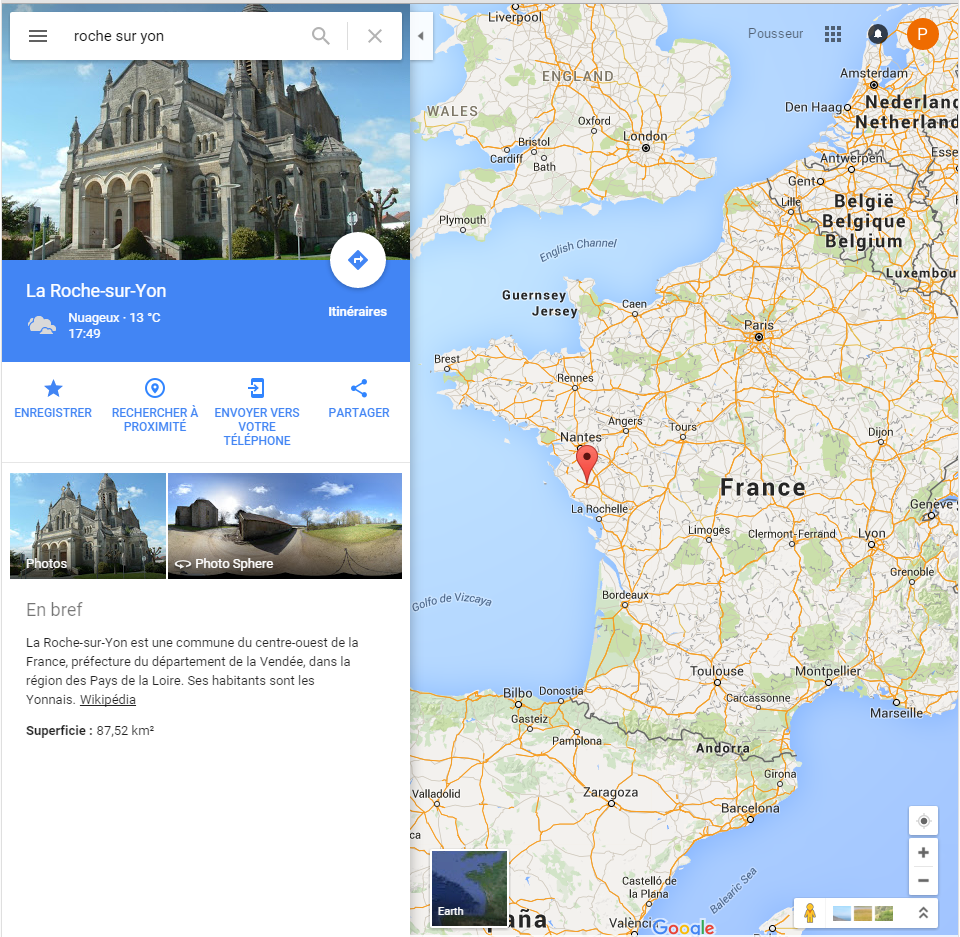
\includegraphics[height=5cm]{img/maps.png}
\end{column}
\end{columns}
\end{frame}


\subsection{Les �preuves}


%%%%%%%%%%%%%%
%%% diapo 5 %%
%%%%%%%%%%%%%%

\begin{frame}
\frametitle{Notre mission cette ann�e :}
\begin{block}{}
\begin{columns}
\begin{column}{0.5\textwidth}
\begin{itemize}
\item Ramasser les roches lunaires
\item Construire une base lunaire
\end{itemize}
\end{column}
\begin{column}{0.5\textwidth}
\begin{itemize}
\item La funny action
\end{itemize}
\end{column}
\end{columns}
\end{block}
\begin{center}
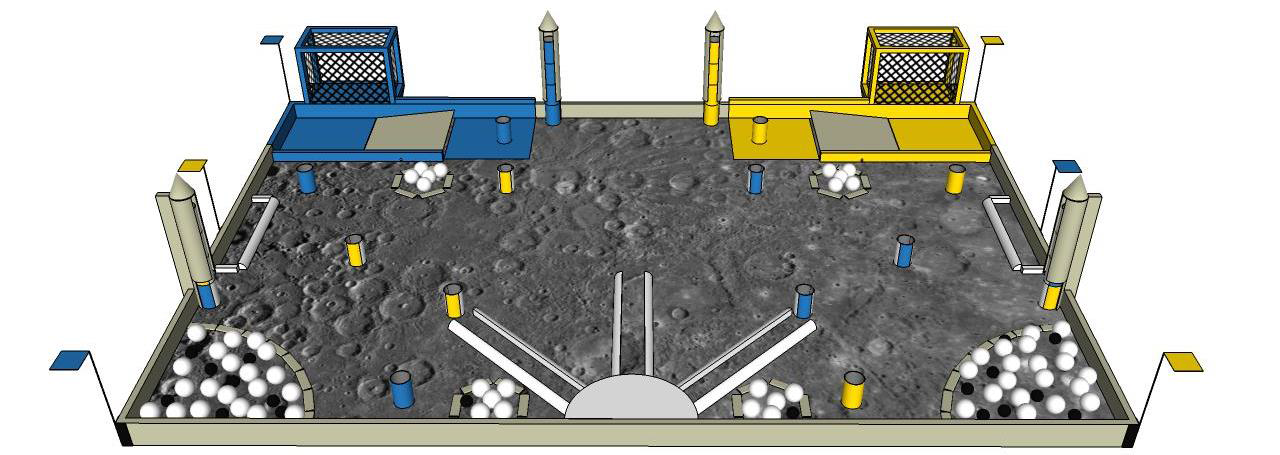
\includegraphics[width=10cm]{img/Table_2017.png} 
\end{center}
\end{frame}



\section{Ing�nieur de demain... D�j� les outils en main !}


%%%%%%%%%%%%%%
%%% diapo 6 %%
%%%%%%%%%%%%%%

\begin{frame}
\frametitle{Nos outils :}
\begin{columns}
\begin{column}{0.4\textwidth}
\begin{block}{}
\begin{itemize}
\item Solidworks
\item Raspberry - Arduino 
\item Latex - Mail 
\item GITHUB
\item ROS 
\end{itemize} 
\end{block}
\begin{center}
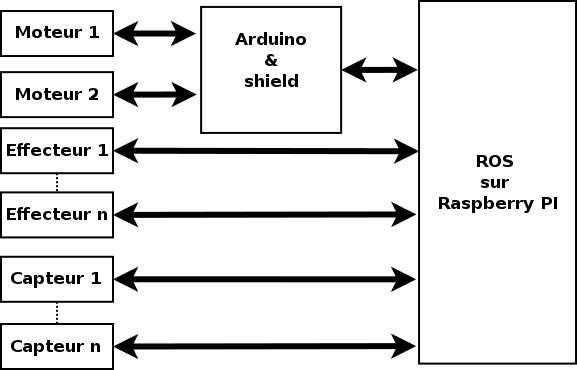
\includegraphics[width=3.5cm]{img/archi_1.png}
\end{center}
\end{column}
\begin{column}{0.5\textwidth}
\begin{center}

\includegraphics[width=3cm]{img/logo_latex.png}\\

\includegraphics[width=4cm]{img/logo_solidworks.jpg}\\
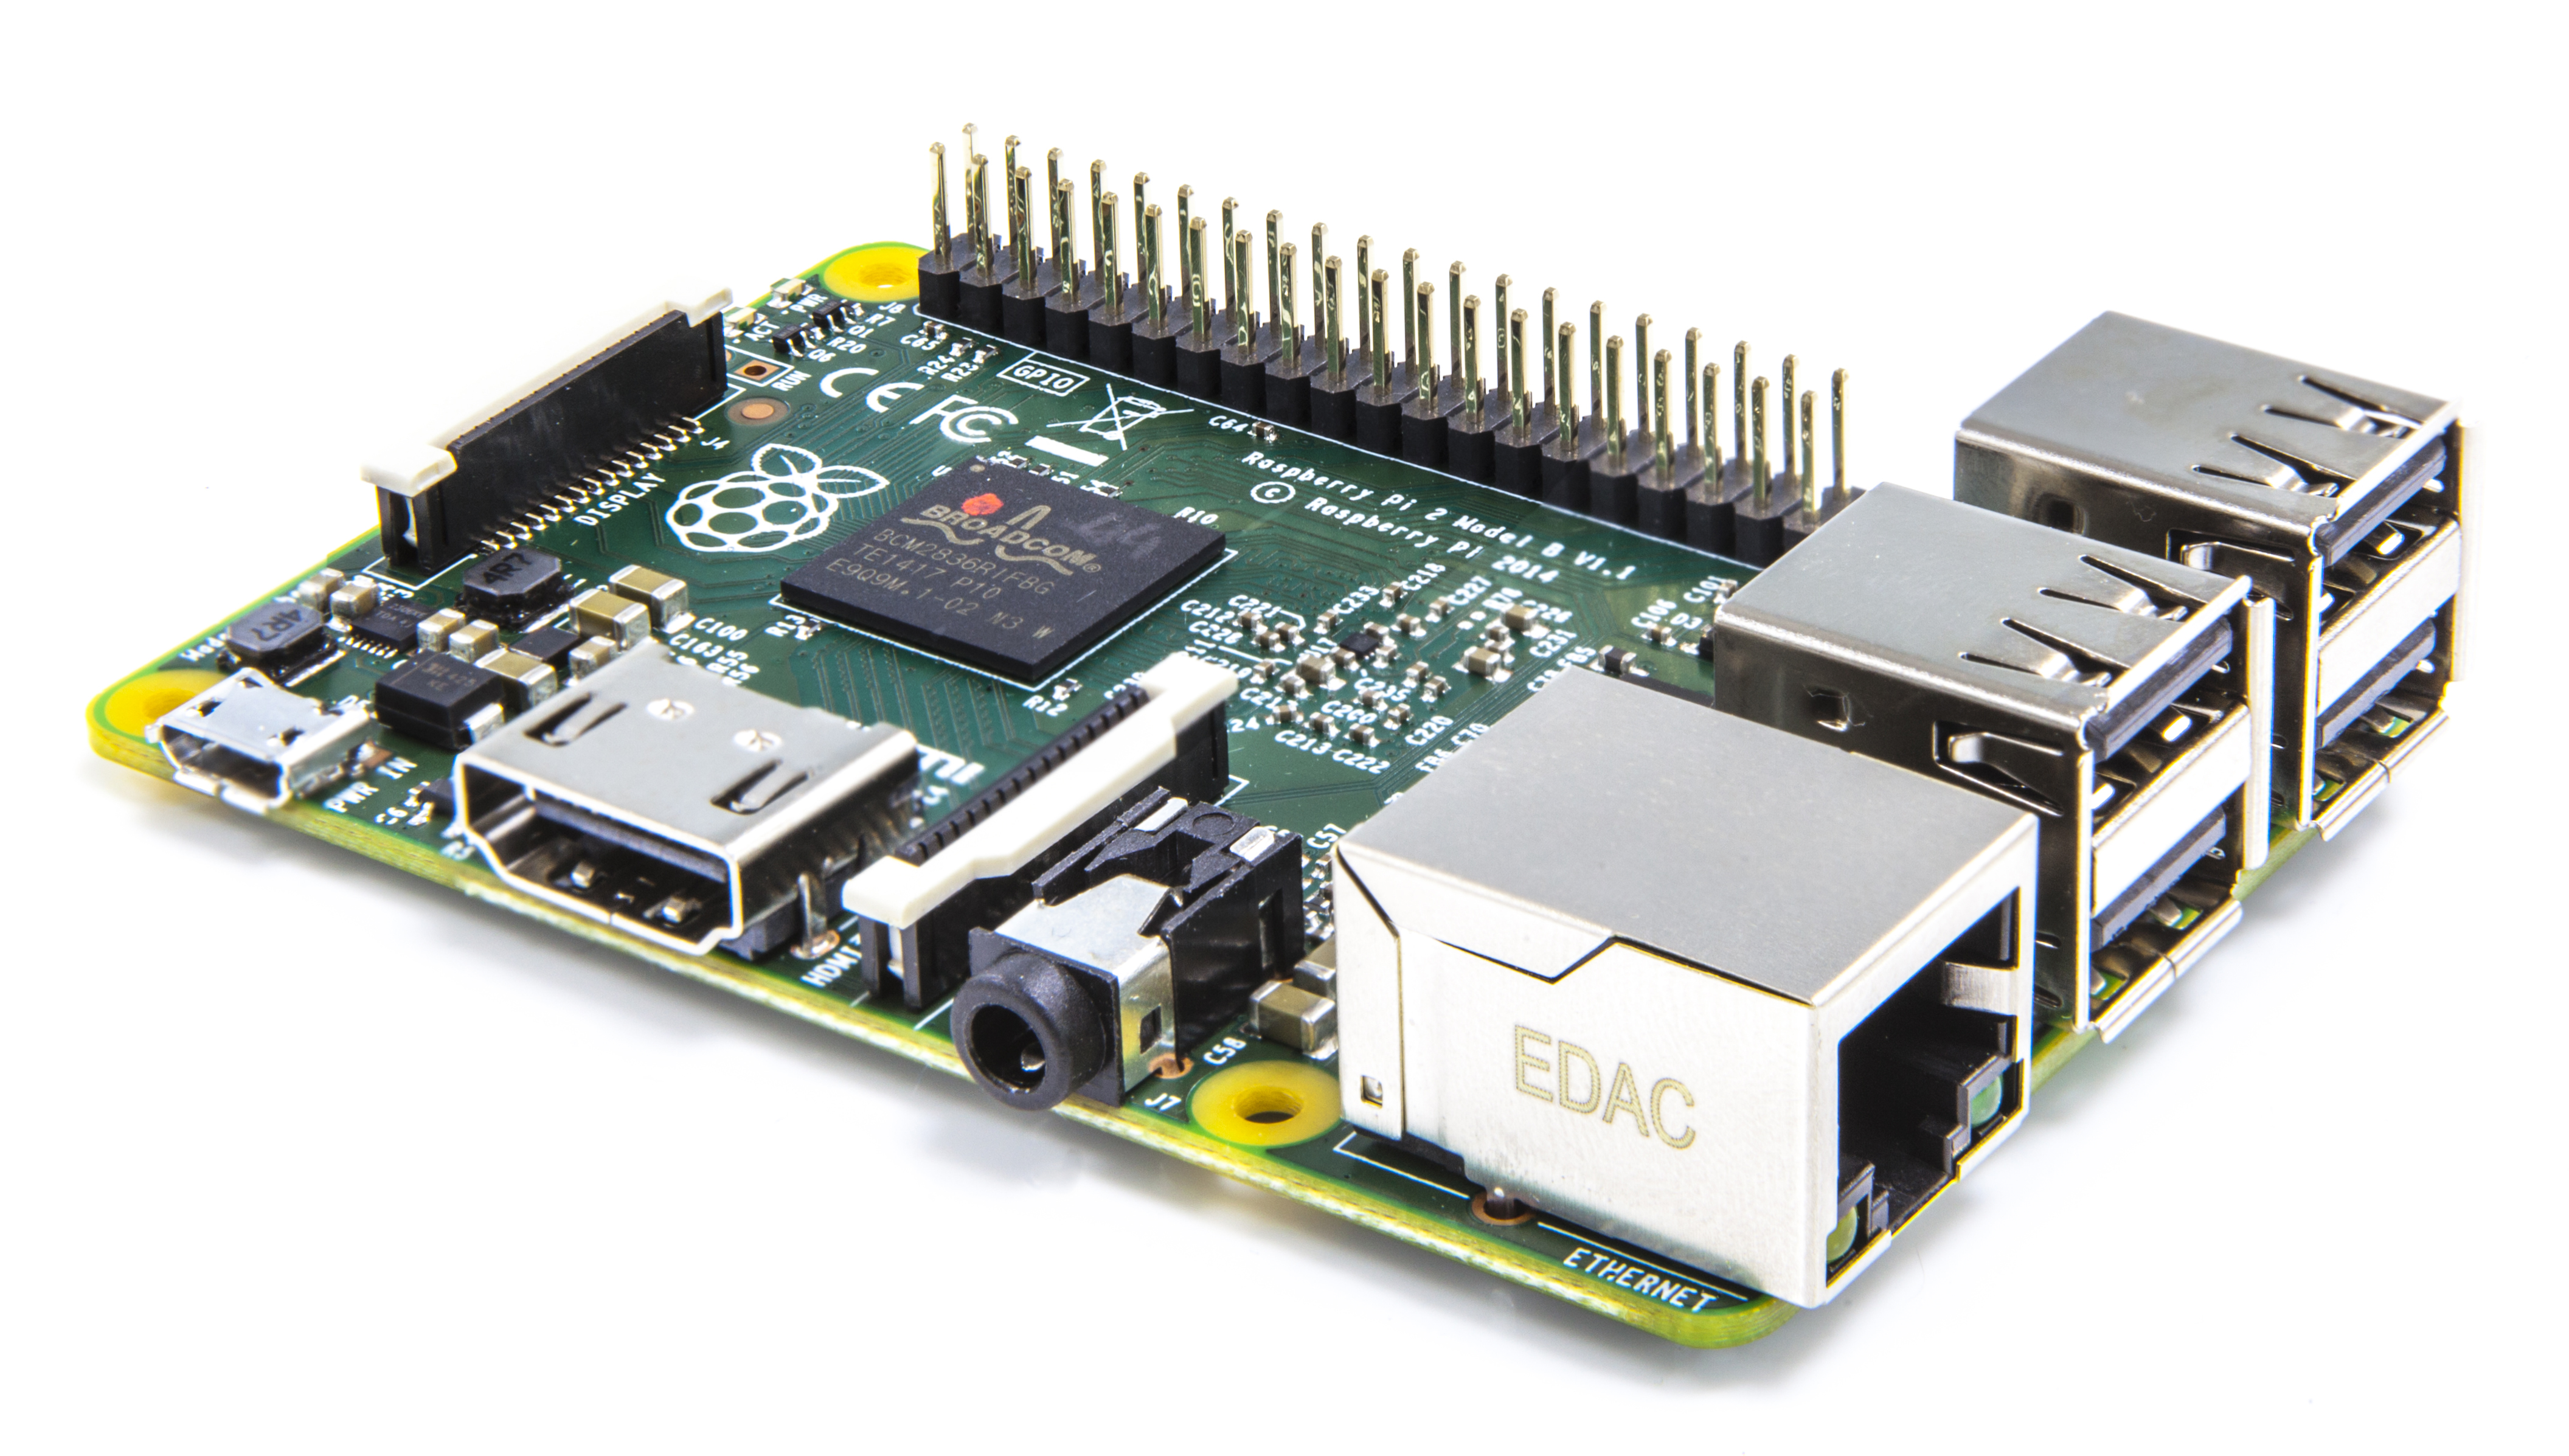
\includegraphics[width=4cm]{img/raspberry.jpeg}\\

\includegraphics[width=4cm]{img/logo_github.jpg}
\end{center}
\end{column}
\end{columns}
\end{frame}


\section{R�partitions des t�ches}


%%%%%%%%%%%%%%
%%% diapo 7 %%
%%%%%%%%%%%%%%

\begin{frame}
\frametitle{Notre graphique des t�ches :}
\begin{block}{}
Utilisation de graphviz
\end{block}
\begin{center}
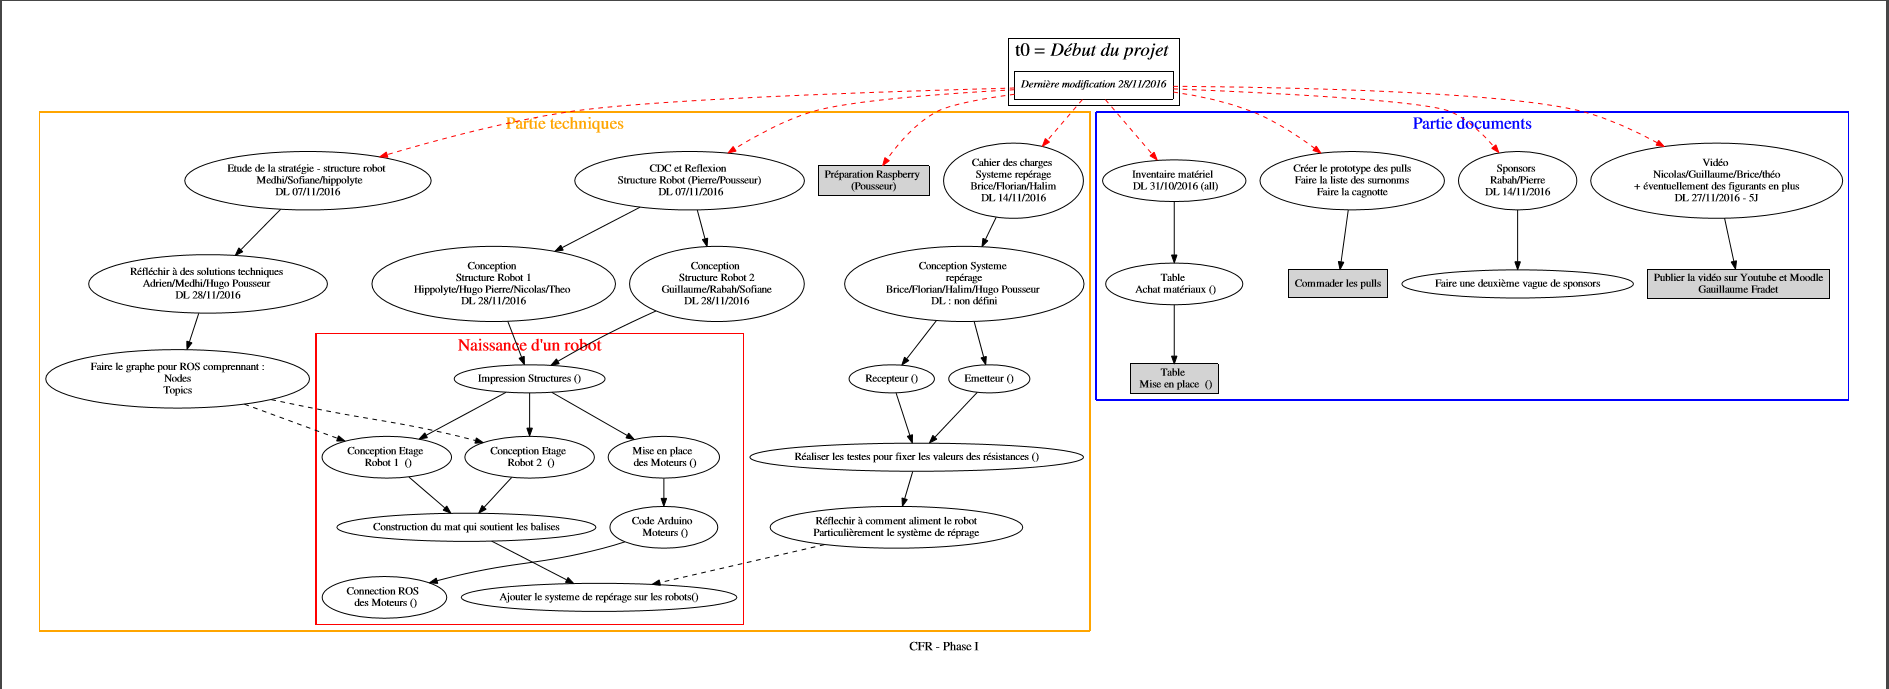
\includegraphics[width=10cm]{img/graphviz.PNG} 
\end{center}
\end{frame}

\section{Avancement du projet}

%%%%%%%%%%%%%%
%%% diapo 8 %%
%%%%%%%%%%%%%%


\begin{frame}
\begin{columns}
\begin{column}{0.7\textwidth}
\begin{center}
	\begin{block}{}
			\begin{itemize}
				\item R�alisation de la table
				\item Prototype syst�me de rep�rage en cours	
				\item Cr�ation du GIT
	 			\item Mod�lisation d'une base roulante + impression
				\item Pr�paration des raspberry Linux + ROS + Python
		 		\item Graphique de la structure de ROS
			\end{itemize}
	\end{block}
	\includegraphics[height=4cm]{img/table_maison.jpg}
	\end{center}
	\end{column}
	\begin{column}{0.3\textwidth}
			\begin{center}
				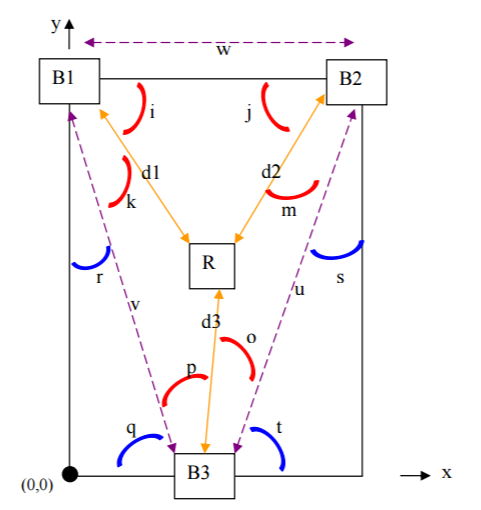
\includegraphics[height=5cm]{img/systeme_reperage.PNG} 	
			\end{center}
		\end{column}
	\end{columns}
	
	 
\end{frame}

\section{Questions}

%%%%%%%%%%%%%%
%%% diapo 9 %%
%%%%%%%%%%%%%%

\begin{frame}
\frametitle{Questions ?}
\begin{center}
L'�quipe CFR vous remercie de votre �coute
\end{center}
\begin{alertblock}{\begin{center}Avez-vous des questions ?\end{center}}
\end{alertblock}
\end{frame}


\end{document}
